% !TeX root = main.tex

\begin{titlepage}

%%%%%%%%%%%%%%%%%%%%%%%%%%%%%%%%%%%%%%%%%%%%%%%%%%%%%%%%%%%%%%%%%%%%%%%%%%%%%%%%
%%% Strona tytułowa
%%%%%%%%%%%%%%%%%%%%%%%%%%%%%%%%%%%%%%%%%%%%%%%%%%%%%%%%%%%%%%%%%%%%%%%%%%%%%%%%

    \begin{center}
	\begin{tabular}{p{107mm} p{9cm}}
	    \begin{minipage}{9cm}
	      \begin{center}
	      Politechnika Warszawska \\
	      Wydział Elektroniki i~Technik Informacyjnych \\
	      Instytut Informatyki
	      \end{center}
	    \end{minipage}
	    &
	    \begin{minipage}{8cm}
	    \begin{flushleft}
	     \footnotesize
	      Rok akademicki 2010/2011
	    \vspace*{2.75\baselineskip}
	    \end{flushleft}
	    \end{minipage} \\
	    \vspace*{1.0\baselineskip}
	\end{tabular}
	
\includegraphics[width=4cm]{../img/logo_pw}
	\par\vspace{\smallskipamount}
	\vspace*{2\baselineskip}{\LARGE PRACA DYPLOMOWA MAGISTERSKA\par}
	\vspace{3\baselineskip}{\LARGE\strut Maciej Stefańczyk\par}
	\vspace*{2\baselineskip}{\huge\bfseries Wykorzystanie informacji z kamery 3D do nawigacji robota mobilnego\par}

	\vspace*{1\baselineskip}
	\hfill\mbox{}\par\vspace*{\baselineskip}\noindent
	\begin{tabular}[b]{@{}p{3cm}@{\ }l@{}}
	    {\large\hfill } & {\large }
	\end{tabular}
	\hfill
	\begin{tabular}[b]{@{}l@{}}
	Opiekun pracy: \\[\smallskipamount]
	{\large dr inż. Tomasz Winiarski}
	\end{tabular}\par
	\vspace*{4\baselineskip}
\begin{tabular}{p{\textwidth}}
    \begin{flushleft}
	\begin{minipage}{7cm}
	Ocena \dotfill
	\par\vspace{1.6\baselineskip}
	\dotfill
	\par\noindent
	\centerline{\footnotesize Podpis Przewodniczącego} \par
	\centerline{\footnotesize Komisji Egzaminu Dyplomowego}\par
	\end{minipage}
    \end{flushleft}
    \end{tabular}
    \end{center}

    %}

	    \cleardoublepage
%%%%%%%%%%%%%%%%%%%%%%%%%%%%%%%%%%%%%%%%%%%%%%%%%%%%%%%%%%%%%%%%%%%%%%%%%%%%%%%%
%%% Dane osobowe
%%%%%%%%%%%%%%%%%%%%%%%%%%%%%%%%%%%%%%%%%%%%%%%%%%%%%%%%%%%%%%%%%%%%%%%%%%%%%%%%
    \newpage\thispagestyle{empty}
    \begin{tabular}{p{5cm} p{11cm}}

    %%% Zdjęcie
    \begin{minipage}{5cm}
    \center
    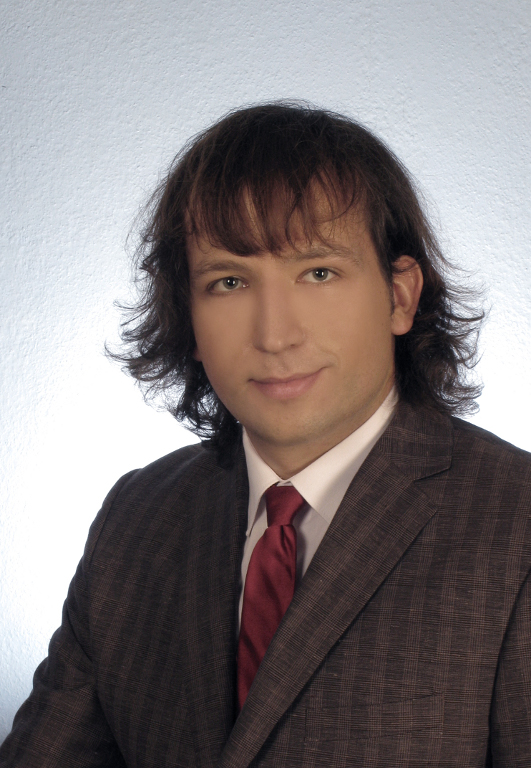
\includegraphics[height=6.5cm,width=4.5cm]{../img/foto}
    \end{minipage}
    &

    %%% Data urodzenia, specjalność itp.
    \begin{minipage}{10cm}

    Specjalność: \hfill Inżynieria Systemów Informatycznych\\
    \\
    Data urodzenia: \hfill 1985.05.04\\
    \\
    Data rozpoczęcia studiów: \hfill 2007.02.21\\

    \end{minipage}

    \end{tabular}

    \vspace*{1\baselineskip}

%%%%%%%%%%%%%%%%%%%%%%%%%%%%%%%%%%%%%%%%%%%%%%%%%%%%%%%%%%%%%%%%%%%%%%%%%%%%%%%%
%%% Życiorys
%%%%%%%%%%%%%%%%%%%%%%%%%%%%%%%%%%%%%%%%%%%%%%%%%%%%%%%%%%%%%%%%%%%%%%%%%%%%%%%%
    \begin{center}
	{\large\bfseries Życiorys}\par\bigskip
    \end{center}

    \indent
    Urodziłem się 4 maja 1985 roku w Warszawie. W~roku 2000 ukończyłem szkołę
    podstawową im.~Kornela Makuszyńskiego, a~w~latach 2000-2004 byłem uczniem
    XXVIII Liceum Ogólnokształcącego im. Jana Kochanowskiego w Warszawie.
    Po ukończeniu szkoły z~wyróżnieniem przez dwa lata studiowałem matematykę na
    wydziale Matematyki i~Nauk Informacyjnych Politechniki Warszawskiej, a~od
    21 lutego 2007 studiuję na wydziale Elektroniki i~Technik Informacyjnych tej
    samej uczelni. W dniu 29 września 2010 uzyskałem tytuł inżyniera z wynikiem
    celującym.
    \par
    \vspace{2\baselineskip}
    \hfill\parbox{15em}{{\small\dotfill}\\[-.3ex]
    \centerline{\footnotesize podpis studenta}}\par

    \vspace{3\baselineskip}

%%%%%%%%%%%%%%%%%%%%%%%%%%%%%%%%%%%%%%%%%%%%%%%%%%%%%%%%%%%%%%%%%%%%%%%%%%%%%%%%
%%% Ocena egzaminu
%%%%%%%%%%%%%%%%%%%%%%%%%%%%%%%%%%%%%%%%%%%%%%%%%%%%%%%%%%%%%%%%%%%%%%%%%%%%%%%%
    \begin{center}
 	{\large\bfseries Egzamin dyplomowy} \par\bigskip\bigskip
    \end{center}
    \par\noindent\vspace{1.5\baselineskip}
    Złożył egzamin dyplomowy w dn. \dotfill
    \par\noindent\vspace{1.5\baselineskip}
    Z wynikiem \dotfill
    \par\noindent\vspace{1.5\baselineskip}
    Ogólny wynik studiów \dotfill
    \par\noindent\vspace{1.5\baselineskip}
    Dodatkowe wnioski i uwagi Komisji \dotfill
    \par\noindent\vspace{1.5\baselineskip}
    \dotfill


	    \cleardoublepage
%%%%%%%%%%%%%%%%%%%%%%%%%%%%%%%%%%%%%%%%%%%%%%%%%%%%%%%%%%%%%%%%%%%%%%%%%%%%%%%%
%%% Streszczenie
%%%%%%%%%%%%%%%%%%%%%%%%%%%%%%%%%%%%%%%%%%%%%%%%%%%%%%%%%%%%%%%%%%%%%%%%%%%%%%%%
    \newpage\thispagestyle{empty}
    %\vspace*{2\baselineskip}
    \begin{center}
	{\large\bfseries Streszczenie}\par\bigskip
    \end{center}

    {\itshape
    Celem niniejszej pracy magisterskiej było zbadanie możliwości wykorzystania
    trójwymiarowej informacji o otoczeniu do nawigacji robota mobilnego. Dodatkowo
    należało rozważyć problem budowania trójwymiarowej mapy otoczenia oraz przedstawić
    wydajną implementację rozwiązania. Docelowy system miał pozwalać na swobodną
    nawigację robota w pomieszczeniach zamkniętych, o nieustrukturyzowanej i
    dynamicznie zmiennej konfiguracji, a także być na tyle elastyczny, aby mógł być
    zastosowany na różnych robotach przy wykorzystaniu różnego rodzaju czujników.
    Drugim zadaniem zrealizowanym w ramach pracy było przygotowanie pełnej platformy
    badawczej pozwalającej na elastyczne testowanie różnych algorytmów związanych
    z nawigacją robotów mobilnych, od przetwarzania danych sensorycznych, przez
    lokalizację i wykrywanie przeszkód, aż po generowanie trajektorii.

    W pracy przedstawiony jest przegląd istniejących rozwiązań umożliwiających
    zbieranie informacji o otoczeniu oraz możliwych metod programowania
    robotów mobilnych. Po wyborze odpowiednich narzędzi scharakteryzowany jest
    dokładniej wykorzystywany sprzęt oraz opisane szczegółowo stworzone poszczególne
    moduły sterowania. Praca kończy się opisem przygotowanych aplikacji testowych
    oraz podsumowaniem uzyskanych rezultatów.
    }
    \vspace*{1\baselineskip}

    \noindent{\bf Słowa kluczowe}: {\itshape nawigacja robotów mobilnych, Kinect, ROS, Elektron }
    \par
    \vspace{4\baselineskip}
    \begin{center}
	{\large\bfseries Abstract}\par\bigskip
    \end{center}
    \noindent{\bf Title}: {\itshape Utilisation of information from the 3D camera for mobile robot navigation}\par
    \vspace*{1\baselineskip}
    {\itshape
    The aim of this thesis was to investigate the possibility of using three-dimensional
    information about the environment for mobile robot navigation. In addition,
    it was necessary to consider the problem of building three-dimensional maps
    of the environment and provide an efficient implementation of the solution.
    The target system had to allow the robot to freely navigate in indoor environments,
    with unstructured and dynamically changing obstacle configuration, and be flexible enough
    so that it can be used for different tasks using wide variety of sensors.
    The second task completed in this study was to prepare a full research platform,
    which allows for testing of various algorithms related to navigation
    of mobile robots, starting from the processing of sensory data, the localization and
    detection of obstacles to the generation of trajectories.

    In this work, there is an overview of existing solutions to gather information about the environment
    and the possible methods of programming mobile robots. After choosing the right
    tools comes characterization of used equipment and various designed control modules.
    Thesis ends with an overview of test applications and and summary of the results.
    }
    \vspace*{1\baselineskip}

    \noindent{\bf Keywords}: {\itshape mobile robot navigation, Kinect, ROS, Elektron}

\end{titlepage}
